\documentclass[12pt]{article}

\usepackage[utf8]{inputenc}
\usepackage[a4paper, margin=1in]{geometry}
\usepackage{booktabs}
\usepackage{physics}
\usepackage{amsmath}
\usepackage{amsfonts}
\usepackage{graphicx}
\usepackage{siunitx}
\usepackage{multirow}

\graphicspath{{./figures}}

\title{Physical Climatology (AES 630) Final}
\author{Mitchell Dodson}
\date{December 6, 2023}

\newcommand*{\problem}[2]{
    \begin{table}[ht]
    \centering
        \begin{tabular}{ | p{.1\linewidth} p{.9\linewidth} | }
            \hline
            \vspace{.3em}\textbf{\large#1:} & \vspace{.3em}\footnotesize{#2}\hspace{.2em}\vspace{.5em} \\ \hline
        \end{tabular}
    \end{table}
}


\newcommand\T{\rule{0pt}{2.6ex}}       % Top strut
\newcommand\B{\rule[-1.2ex]{0pt}{0pt}} % Bottom strut

\begin{document}

\vspace{-2em}

\maketitle

\vspace{-2em}

\section{EBM Problem}

\begin{figure}[h!]
    \centering
    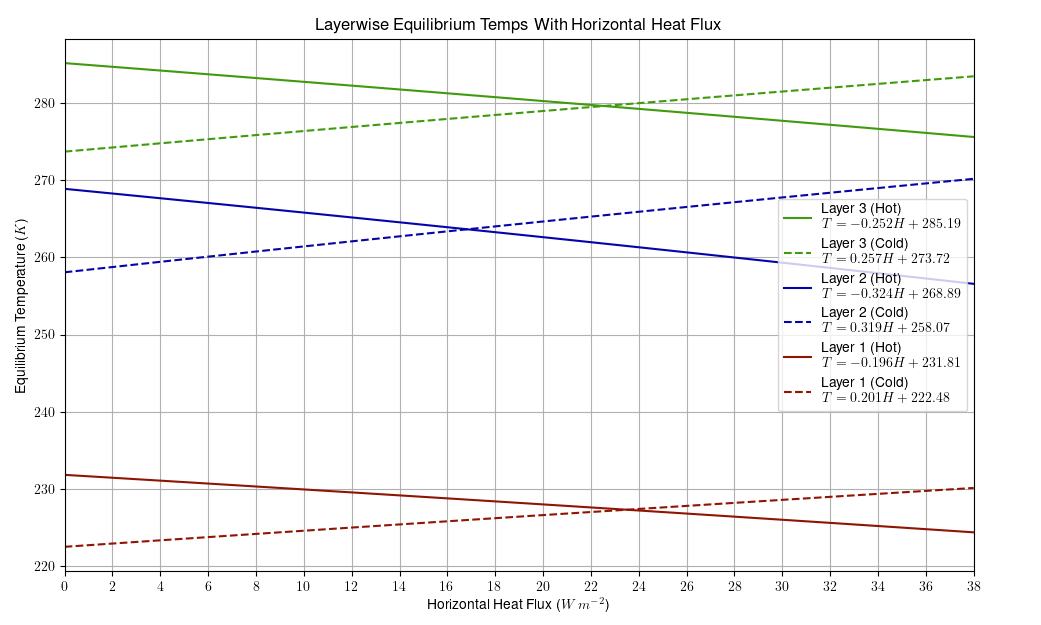
\includegraphics[width=.98\linewidth]{q1.png}

    \vspace{1em}

    \begin{tabular}{c | c c c | c c c}
        & Layer 1 & Layer 2 & Layer 3 & $\frac{dT_1}{dH}$ & $\frac{dT_2}{dH}$ & $\frac{dT_3}{dH}$ \B\\
        \hline
        Hot World & 231.809 & 268.891 & 285.192 & -0.196 & -0.324 & -0.252 \T\\
        Cold World & 222.480 & 258.070 & 273.715 & 0.201 & 0.319 & 0.257 \\
    \end{tabular}

    \caption{Equilibrium temperatures of ``hot world'' with $Q_H = 330\,\si{W.m^{-2}}$ and ``cold world'' with $Q_C = 280\,\si{W.m^{-2}}$ as horizontal heat flux from the hot to the cold world's troposphere increases up to $38\,\si{W.m^{-2}}$. The table shows the initial layerwise temperatures as well as their linear rates of change with respect to the heat flux.}
    \label{q1}
\end{figure}

\begin{equation}\label{conduit}
    \begin{split}
        T_{3C} &= T_{3H} \\
        -0.252\,H + 285.19 &= 0.257\,H + 273.72 \\
        H &= 22.53\,\si{W.m^{-2}}\\
    \end{split}
\end{equation}

Figure \ref{q1} shows the effects on each layer's equilibrium temperature as the exchange of heat between the hot and cold worlds increases, and Equation \ref{conduit} sets each planet's linear approximation of the surface temperature response equal to each other in order to determine their intersection. My results show that the conduit between each world's troposphere must transmit $H=22.53\,\si{W.m^{-2}}$ of heat flux in order to maintain the same surface temperature between the two systems.

\begin{equation}\label{instability}
    \begin{split}
        T_{3H} = T_{3C} &= 0.257 \cdot 22.53 + 273.72 = 279.51\,\si{K} \\
        T_{2H} &= -0.324 \cdot 22.53 + 268.89 = 261.59\,\si{K} \\
        T_{2C} &= 0.319 \cdot 22.53 + 258.07 = 265.26\,\si{K} \\
    \end{split}
\end{equation}

Equation \ref{instability} shows the equilibrium temperatures of layers 2 and 3 for both planets at the surface temperature intersection, given their linear approximations. These suggest that in the cold planet the temperature difference between the surface and the troposphere is $T_{3C}-T_{2C} = 14.25\,\si{K}$, and in the hot planet the temperature difference is $T_{3H}-T_{2H} = 17.92\,\si{K}$. Assuming layer 2 is the same altitude from the surface for both planets, this indicates that the addition of heat to the cold planet's troposphere weakens its lapse rate relative to the hot planet. The result is that less potential energy is available for buoyant air parcels to be lofted from the cold planet, which correlates with less overall vertical heat flux for that planet. The inverse is true for the hot planet, which has a relatively steep lapse rate that may enhance the rate at which vertical heat flux redistributes energy from the surface layers to the troposphere. Furthermore, the absolute magnitudes of $\frac{dT_2}{dH}$ are greater than those of $\frac{dT_3}{dH}$ in both planets' cases. This suggests that after implementing the heat conduit, the hydrostatic instability of the hot planet increases and the cold planet becomes more stable compared to their original lapse rates.

\section{Climate Sensitivity and Politics}

\noindent\textbf{Part A}

\begin{equation}\label{sb1}
    T_s = \sqrt[4]{\frac{S_0 (1-\alpha_p)}{4 \sigma}} = \sqrt[4]{\frac{1365 (1-0.31)}{4 \sigma}} = 253.85\,\si{K}
\end{equation}

\begin{equation}\label{sb2}
    \frac{d E}{d T_s} =  \frac{d}{dT_s}(\sigma T_s^4) = 4\sigma T_s^3 = 4 \sigma (253.85\,\si{K})^3 = 3.71\,\si{W.m^{-2}.K^{-1}}
\end{equation}

\begin{equation}\label{sb3}
    \lambda_R = \frac{d T_s}{d E} = \frac{1}{3.71} = 0.2695\,\si{K.(W.m^{-2})^{-1}}
\end{equation}

The Stefan-Boltzmann feedback with no atmosphere describes a planetary energy system with a surface temperature that only depends on the amount of insolation that is attenuated by the surface, which is modulated by the solar constant $S_0 = 1365\,\si{W.m^{-2}}$ and the surface's albedo (and by extension its absorptivity/emissivity). Equation \ref{sb1} shows that the surface temperature in this model is $253.85\,\si{K}$ assuming Earth's approximate albedo of $\alpha_p = 0.31$.

Equation \ref{sb2} characterizes the change in the planet's radiant exitance with respect to surface temperature in terms of the Stefan-Boltzmann law. If we were modeling the actual radiative power of the surface it would be more appropriate to include an emissivity coefficient $\epsilon_p = 1-0.31 = 0.69$, however for the sake of this question I assume the surface radiates as a blackbody as a standard for reference. Inverting this equation to express the change in surface temperature with respect to the radiant exitance, Equation \ref{sb3} shows that the climate sensitivity given only the Stefan-Boltzmann feedback for a planet with no atmosphere is $\lambda_R = 0.2695$.

\vspace{2em}\noindent\textbf{Part B}

\begin{equation}
    \sigma T_e^4 = \sigma T_a^4 = \frac{S_0}{4}(1-\alpha_p)
\end{equation}

In a planetary system with a single thermally-opaque atmospheric layer,

\begin{equation}
\end{equation}

\end{document}

\begin{figure}[h!]\label{q1q2}
    \centering
    \begin{tabular}{ r | c | c c c}
        Model & Metric & Layer 1 & Layer 2 & Surface \T\B\\
        %\hline
        %\multicolumn{4}{c}{EBM3} \\
        \hline
        \multirow{2}*{EBM3$_0$} &
        Absorption ($\si{W.m^{-2}}$) & 8.714 & 59.969 & 170.158 \T\\
        & Temperature ($\si{K}$) & 233.716 & 269.503 & 308.461 \B\\
        %\hline
        %\multicolumn{4}{c}{EBM3 with Heat Flux} \\
        \hline
        \multirow{2}*{EBM3$_{HF}$} &
        Absorption ($\si{W.m^{-2}}$) & 8.713 & 158.859 & 71.268 \T\\
        & Temperature ($\si{K}$) & 233.716 & 271.120 & 287.295 \B\\
        \hline
        %\multicolumn{4}{c}{Kiehl and Trenberth 2} \\
        %\hline
        \multirow{2}*{K$\&$H 2} &
        Absorption ($\si{W.m^{-2}}$) & 10.547 & 174.976 & 48.809 \T\\
        & Temperature ($\si{K}$) & 243.985 & 286.226 & 286.587 \B\\
    \end{tabular}
    \caption{Layerwise equilibrium temperature and absorption of shortwave solar and heat flux energy for each of the coefficient sets of the 3-layer energy-based model. The absorption results for EBM3$_{HF}$ and Kiehl$\&$Trenberth 2 (K$\&$H 2) include heat flux from the surface to layer 2 such that HF$:=.29Q$ for average solar irradiance $Q=341\,\si{W.m^{-2}}$.}
\end{figure}
